% questions.tex —— 2020 年·全国Ⅲ卷·理科 · 题目内容片段（无答案）
% 由 tools/generate_projects.py 依来源总账自 2020/2020_数学真题_全国3理_试题.md 生成，勿手改（改源 MD 后重跑）


\begin{gknotice}
\textbf{来源说明}：本题面依据固定源 PDF 的两页 A3 题面逐题转录，原卷印刷页码为 1125、1126。第 1125 面为选择题 1—12、填空题 13—16 与解答题 17、18；第 1126 面为解答题 19—23。全卷三处节头依次为「一、选择题」「二、填空题」「三、解答题」，题号与索引一致；所有数值、分式、根号与上下标均回原页 300—600 dpi 核对。

\textbf{解析归属}：固定源不附答案或解析；配套答案与解析均由本库按本题面独立复算（等级 D，非官方）。

\textbf{选做说明}：原卷第 22、23 题按选修模块二选一命制，题面未另加模块标题。本库全部收录，并以【A】标记第 22 题（选修 4—4 坐标系与参数方程）、【B】标记第 23 题（选修 4—5 不等式选讲），便于检索。

\textbf{图形说明}：第 8 题的三视图、第 19 题的长方体由项目内 TikZ 矢量源重绘；第 20 题椭圆原页无图；其余各题原页无图。

\textbf{校勘}：第 4 题原页「流行病学领城」显系「领域」之误，转录时径改为「领域」，其余文字照录。
\end{gknotice}

\gkpart{一、选择题}

\begin{question}
\gkti{1}已知集合 $A=\{(x,y)\mid x,y\in\mathbf N^*,\ y\geqslant x\}$，$B=\{(x,y)\mid x+y=8\}$，则 $A\cap B$ 中元素的个数为\mbox{（　　）}

（A）$2$；（B）$3$；（C）$4$；（D）$6$。

\end{question}
\begin{question}
\gkti{2}复数 $\dfrac1{1-3\mathrm i}$ 的虚部是\mbox{（　　）}

（A）$-\dfrac3{10}$；（B）$-\dfrac1{10}$；（C）$\dfrac1{10}$；（D）$\dfrac3{10}$。

\end{question}
\begin{question}
\gkti{3}在一组样本数据中，$1$，$2$，$3$，$4$ 出现的频率分别为 $p_1$，$p_2$，$p_3$，$p_4$，且 $\sum\limits_{i=1}^4p_i=1$，则下面四种情形中，对应样本的标准差最大的一组是\mbox{（　　）}

（A）$p_1=p_4=0.1$，$p_2=p_3=0.4$；（B）$p_1=p_4=0.4$，$p_2=p_3=0.1$；（C）$p_1=p_4=0.2$，$p_2=p_3=0.3$；（D）$p_1=p_4=0.3$，$p_2=p_3=0.2$。

\end{question}
\begin{question}
\gkti{4}Logistic 模型是常用数学模型之一，可应用于流行病学领域。有学者根据公布数据建立了某地区新冠肺炎累计确诊病例数 $I(t)$（$t$ 的单位：天）的 Logistic 模型：$I(t)=\dfrac K{1+\mathrm e^{-0.23(t-53)}}$，其中 $K$ 为最大确诊病例数。当 $I(t^*)=0.95K$ 时，标志着已初步遏制疫情，则 $t^*$ 约为（$\ln19\approx3$）\mbox{（　　）}

（A）$60$；（B）$63$；（C）$66$；（D）$69$。

\end{question}
\begin{question}
\gkti{5}设 $O$ 为坐标原点，直线 $x=2$ 与抛物线 $C:y^2=2px$（$p>0$）交于 $D$，$E$ 两点。若 $OD\perp OE$，则 $C$ 的焦点坐标为\mbox{（　　）}

（A）$\left(\dfrac14,0\right)$；（B）$\left(\dfrac12,0\right)$；（C）$(1,0)$；（D）$(2,0)$。

\end{question}
\begin{question}
\gkti{6}已知向量 $\boldsymbol a$，$\boldsymbol b$ 满足 $|\boldsymbol a|=5$，$|\boldsymbol b|=6$，$\boldsymbol a\cdot\boldsymbol b=-6$，则 $\cos\langle\boldsymbol a,\boldsymbol a+\boldsymbol b\rangle=$\mbox{（　　）}

（A）$-\dfrac{31}{35}$；（B）$-\dfrac{19}{35}$；（C）$\dfrac{17}{35}$；（D）$\dfrac{19}{35}$。

\end{question}
\begin{question}
\gkti{7}在 $\triangle ABC$ 中，$\cos C=\dfrac23$，$AC=4$，$BC=3$，则 $\cos B=$\mbox{（　　）}

（A）$\dfrac19$；（B）$\dfrac13$；（C）$\dfrac12$；（D）$\dfrac23$。

\Needspace{0.4\textheight}
\end{question}
\begin{question}
\gkti{8}下图为某几何体的三视图，则该几何体的表面积是\mbox{（　　）}

（A）$6+4\sqrt2$；（B）$4+4\sqrt2$；（C）$6+2\sqrt3$；（D）$4+2\sqrt3$。
\nopagebreak[4]
\begin{center}% 2020 全国Ⅲ卷 理8：某几何体的三视图
% 来源 PDF：普通高考/2020/2020全国3理(云南,广西,贵州,西藏,四川).pdf 第 1 页（A3 横排），印面 1125，第 8 题题干下方
% 结构（按原页矢量数据换算）：主视图、左视图、俯视图均为腰长 2 的等腰直角三角形；
%   主视图直角在右下，左视图直角在左下，俯视图直角在右上。三视图的直角互相对应，
%   故该几何体是三条两两垂直的棱长均为 2 的四面体。
% 尺寸标注：原页只在主视图底边、主视图右边、俯视图右边标出「2」，此处照录。
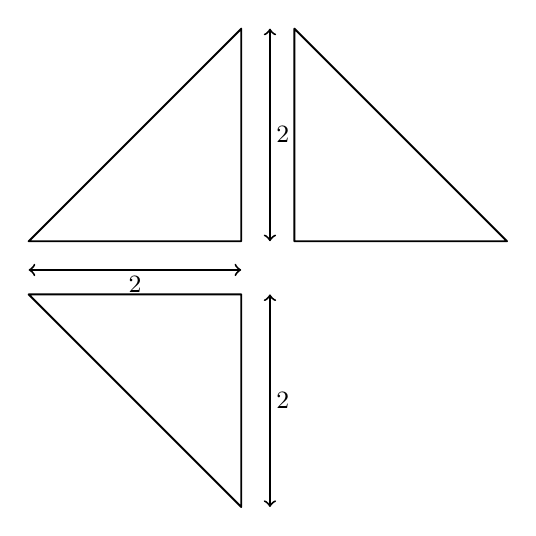
\begin{tikzpicture}[line width=0.7pt, font=\small,
  x=1.35cm, y=1.35cm, line cap=round, line join=round]

  % 主视图：直角边 2 与 2，直角在右下
  \draw (0,0) -- (2,0) -- (2,2) -- cycle;

  % 左视图：直角边 2 与 2，直角在左下
  \draw (2.5,0) -- (4.5,0) -- (2.5,2) -- cycle;

  % 俯视图：直角边 2 与 2，直角在右上
  \draw (0,-0.5) -- (2,-0.5) -- (2,-2.5) -- cycle;

  % 尺寸标注
  \draw[<->] (0,-0.27) -- (2,-0.27) node[midway, below, inner sep=2pt] {$2$};
  \draw[<->] (2.27,0) -- (2.27,2) node[midway, right, inner sep=2pt] {$2$};
  \draw[<->] (2.27,-0.5) -- (2.27,-2.5) node[midway, right, inner sep=2pt] {$2$};
\end{tikzpicture}
\end{center}
\nopagebreak[4]
\end{question}
\begin{question}
\gkti{9}已知 $2\tan\theta-\tan\left(\theta+\dfrac\pi4\right)=7$，则 $\tan\theta=$\mbox{（　　）}

（A）$-2$；（B）$-1$；（C）$1$；（D）$2$。

\end{question}
\begin{question}
\gkti{10}若直线 $l$ 与曲线 $y=\sqrt x$ 和 $x^2+y^2=\dfrac15$ 都相切，则 $l$ 的方程为\mbox{（　　）}

（A）$y=2x+1$；（B）$y=2x+\dfrac12$；（C）$y=\dfrac12x+1$；（D）$y=\dfrac12x+\dfrac12$。

\end{question}
\begin{question}
\gkti{11}设双曲线 $C:\dfrac{x^2}{a^2}-\dfrac{y^2}{b^2}=1$（$a>0$，$b>0$）的左、右焦点分别为 $F_1$，$F_2$，离心率为 $\sqrt5$。$P$ 是 $C$ 上一点，且 $F_1P\perp F_2P$。若 $\triangle PF_1F_2$ 的面积为 $4$，则 $a=$\mbox{（　　）}

（A）$1$；（B）$2$；（C）$4$；（D）$8$。

\end{question}
\begin{question}
\gkti{12}已知 $5^5<8^4$，$13^4<8^5$。设 $a=\log_53$，$b=\log_85$，$c=\log_{13}8$，则\mbox{（　　）}

（A）$a<b<c$；（B）$b<a<c$；（C）$b<c<a$；（D）$c<a<b$。

\end{question}
\gkpart{二、填空题}

\begin{question}
\gkti{13}若 $x$，$y$ 满足约束条件 $\begin{cases}x+y\geqslant0,\\2x-y\geqslant0,\\x\leqslant1,\end{cases}$ 则 $z=3x+2y$ 的最大值为\gkblank{}。

\end{question}
\begin{question}
\gkti{14}$\left(x^2+\dfrac2x\right)^6$ 的展开式中常数项是\gkblank{}。（用数字作答）

\end{question}
\begin{question}
\gkti{15}已知圆锥的底面半径为 $1$，母线长为 $3$，则该圆锥内半径最大的球的体积为\gkblank{}。

\end{question}
\begin{question}
\gkti{16}关于函数 $f(x)=\sin x+\dfrac1{\sin x}$ 有如下四个命题：

① $f(x)$ 的图象关于 $y$ 轴对称；

② $f(x)$ 的图象关于原点对称；

③ $f(x)$ 的图象关于直线 $x=\dfrac\pi2$ 对称；

④ $f(x)$ 的最小值为 $2$。

其中所有真命题的序号是\gkblank{}。

\end{question}
\gkpart{三、解答题}

\begin{question}
\gkti{17}设数列 $\{a_n\}$ 满足 $a_1=3$，$a_{n+1}=3a_n-4n$。

（1） 计算 $a_2$，$a_3$，猜想 $\{a_n\}$ 的通项公式并加以证明；

（2） 求数列 $\{2^na_n\}$ 的前 $n$ 项和 $S_n$。

\end{question}
\begin{question}
\gkti{18}某学生兴趣小组随机调查了某市 $100$ 天中每天的空气质量等级和当天到某公园锻炼的人次，整理数据得到下表（单位：天）：

\begin{center}
\begin{tabular}{cccc}
\toprule
空气质量等级／锻炼人次 & $[0,200]$ & $(200,400]$ & $(400,600]$ \\
\midrule
$1$（优） & $2$ & $16$ & $25$ \\
$2$（良） & $5$ & $10$ & $12$ \\
$3$（轻度污染） & $6$ & $7$ & $8$ \\
$4$（中度污染） & $7$ & $2$ & $0$ \\
\bottomrule
\end{tabular}
\end{center}

（1） 分别估计该市一天的空气质量等级为 $1$，$2$，$3$，$4$ 的概率；

（2） 求一天中到该公园锻炼的平均人次的估计值（同一组中的数据用该组区间的中点值为代表）；

（3） 若某天的空气质量等级为 $1$ 或 $2$，则称这天“空气质量好”；若某天的空气质量等级为 $3$ 或 $4$，则称这天“空气质量不好”。根据所给数据，完成下面的 $2\times2$ 列联表，并根据列联表，判断是否有 $95\%$ 的把握认为一天中到该公园锻炼的人次与该市当天的空气质量有关？

\begin{center}
\begin{tabular}{ccc}
\toprule
 & 人次 $\leqslant400$ & 人次 $>400$ \\
\midrule
空气质量好 &  &  \\
空气质量不好 &  &  \\
\bottomrule
\end{tabular}
\end{center}

\Needspace{10\baselineskip}
附：$K^2=\dfrac{n(ad-bc)^2}{(a+b)(c+d)(a+c)(b+d)}$，

\begin{center}
\begin{tabular}{cccc}
\toprule
$P(K^2\geqslant k)$ & $0.050$ & $0.010$ & $0.001$ \\
\midrule
$k$ & $3.841$ & $6.635$ & $10.828$ \\
\bottomrule
\end{tabular}
\end{center}

\Needspace{0.4\textheight}
\end{question}
\begin{question}
\gkti{19}如图，在长方体 $ABCD-A_1B_1C_1D_1$ 中，点 $E$，$F$ 分别在棱 $DD_1$，$BB_1$ 上，且 $2DE=ED_1$，$BF=2FB_1$。

（1） 证明：点 $C_1$ 在平面 $AEF$ 内；

（2） 若 $AB=2$，$AD=1$，$AA_1=3$，求二面角 $A-EF-A_1$ 的正弦值。
\nopagebreak[4]
\begin{center}% 2020 全国Ⅲ卷 理19：长方体 ABCD-A1B1C1D1，E 在 DD1、F 在 BB1 上
% 来源 PDF：普通高考/2020/2020全国3理(云南,广西,贵州,西藏,四川).pdf 第 2 页（A3 横排），印面 1126，第 19 题题干下方
% 结构（按原页矢量数据换算）：ABCD 为上底面，A1B1C1D1 为下底面；A 在前右、B 在后右、
%   C 在后左、D 在前左；AD = 1 为图面横向单位，AA1 = 3 为竖向单位，AB = 2 沿 45° 方向
%   以半长画出（原页即如此，AB 与 AD 在图面上等长）。
%   E 在棱 DD1 上且 2DE = ED1（自 D 向下三分之一处），F 在棱 BB1 上且 BF = 2FB1（自 B 向下三分之二处）。
% 实线：DA、AB、BC、CD、DD1、AA1、BB1、D1A1、A1B1 以及 AE、AF、A1E、A1F；
% 虚线：CC1（被遮挡的棱）、C1D1 与 C1B1（被遮挡的底棱）以及体内线段 EF。
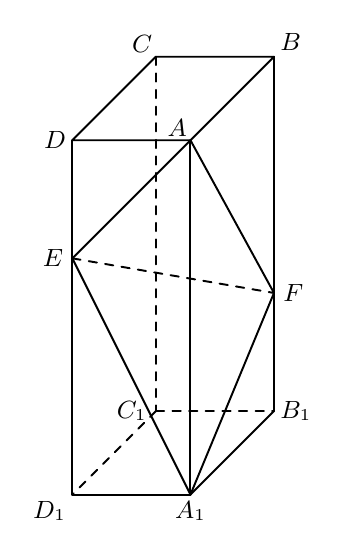
\begin{tikzpicture}[line width=0.7pt, font=\small,
  x=1.5cm, y=1.5cm, line cap=round, line join=round]

  % 顶点
  \coordinate (D)  at (0,3);
  \coordinate (A)  at (1,3);
  \coordinate (C)  at (0.70711,3.70711);
  \coordinate (B)  at (1.70711,3.70711);
  \coordinate (D1) at (0,0);
  \coordinate (A1) at (1,0);
  \coordinate (C1) at (0.70711,0.70711);
  \coordinate (B1) at (1.70711,0.70711);

  % E、F 按定比取点
  \coordinate (E) at (0,2);
  \coordinate (F) at (1.70711,1.70711);

  % 上底面
  \draw (D) -- (A) -- (B) -- (C) -- cycle;

  % 可见棱
  \draw (D) -- (D1);
  \draw (A) -- (A1);
  \draw (B) -- (B1);
  \draw (D1) -- (A1);
  \draw (A1) -- (B1);

  % 题设线段
  \draw (A) -- (E);
  \draw (A) -- (F);
  \draw (A1) -- (E);
  \draw (A1) -- (F);

  % 被遮挡的棱与体内线段
  \draw[dashed] (C) -- (C1);
  \draw[dashed] (C1) -- (D1);
  \draw[dashed] (C1) -- (B1);
  \draw[dashed] (E) -- (F);

  % 顶点标注
  \node[above left,  inner sep=1pt] at (C)  {$C$};
  \node[above right, inner sep=2pt] at (B)  {$B$};
  \node[left,        inner sep=2pt] at (D)  {$D$};
  \node[above left,  inner sep=1pt] at (A)  {$A$};
  \node[left,        inner sep=3pt] at (E)  {$E$};
  \node[right,       inner sep=3pt] at (F)  {$F$};
  \node[below left,  inner sep=2pt] at (D1) {$D_1$};
  \node[below,       inner sep=2pt] at (A1) {$A_1$};
  \node[left,        inner sep=3pt] at (C1) {$C_1$};
  \node[right,       inner sep=2pt] at (B1) {$B_1$};
\end{tikzpicture}
\end{center}
\nopagebreak[4]
\end{question}
\begin{question}
\gkti{20}已知椭圆 $C:\dfrac{x^2}{25}+\dfrac{y^2}{m^2}=1$（$0<m<5$）的离心率为 $\dfrac{\sqrt{15}}4$，$A$，$B$ 分别为 $C$ 的左、右顶点。

（1） 求 $C$ 的方程；

（2） 若点 $P$ 在 $C$ 上，点 $Q$ 在直线 $x=6$ 上，且 $|BP|=|BQ|$，$BP\perp BQ$，求 $\triangle APQ$ 的面积。

\end{question}
\begin{question}
\gkti{21}设函数 $f(x)=x^3+bx+c$，曲线 $y=f(x)$ 在点 $\left(\dfrac12,f\left(\dfrac12\right)\right)$ 处的切线与 $y$ 轴垂直。

（1） 求 $b$；

（2） 若 $f(x)$ 有一个绝对值不大于 $1$ 的零点，证明：$f(x)$ 所有零点的绝对值都不大于 $1$。

\end{question}
\begin{question}
\gkti{22}\textbf{【A】（选修 4—4：坐标系与参数方程）} 在直角坐标系 $xOy$ 中，曲线 $C$ 的参数方程为 $\begin{cases}x=2-t-t^2,\\y=2-3t+t^2\end{cases}$（$t$ 为参数且 $t\neq1$），$C$ 与坐标轴交于 $A$，$B$ 两点。

（1） 求 $|AB|$；

（2） 以坐标原点为极点，$x$ 轴正半轴为极轴建立极坐标系，求直线 $AB$ 的极坐标方程。

\end{question}
\begin{question}
\gkti{23}\textbf{【B】（选修 4—5：不等式选讲）} 设 $a$，$b$，$c\in\mathbf R$，$a+b+c=0$，$abc=1$。

（1） 证明：$ab+bc+ca<0$；

（2） 用 $\max\{a,b,c\}$ 表示 $a$，$b$，$c$ 中的最大值，证明：$\max\{a,b,c\}\geqslant\sqrt[3]4$。

\end{question}